\documentclass[tikz,border=4pt]{standalone}
\usepackage{amsmath}
\usepackage{pgfplots}
\pgfplotsset{compat=1.18}

\begin{document}
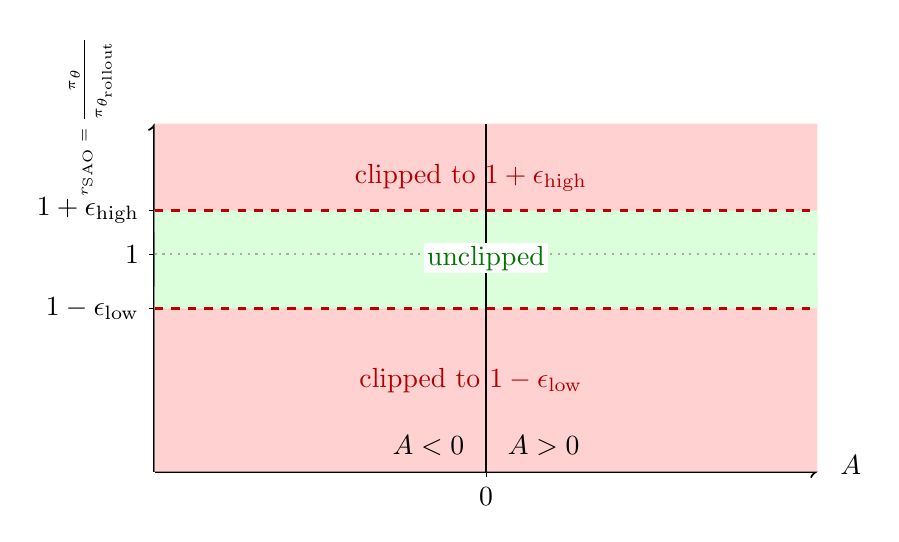
\begin{tikzpicture}
\begin{axis}[
  width=10cm,
  height=6cm,
  xmin=-2.2,
  xmax=2.2,
  ymin=0,
  ymax=1.6,
  axis lines=left,
  axis line style={->, thick},
  xlabel={$A$},
  ylabel={\tiny{$r_{\mathrm{SAO}}=\dfrac{\pi_\theta}{\pi_{\theta_{\mathrm{rollout}}}}$}},
  xlabel style={at={(axis description cs:1.02,0.02)}, anchor=west},
  ylabel style={at={(axis description cs:-0.05,1.02)}, anchor=south, font=\small},
  xtick={0},
  xticklabels={$0$},
  ytick={0.75,1,1.20},
  yticklabels={$1-\epsilon_{\mathrm{low}}$,$1$,$1+\epsilon_{\mathrm{high}}$},
  tick style={black},
  enlargelimits=false,
  clip=false
]

% SAO applies the clip operator directly to the behavior-policy ratio,
% so clipping depends only on r_SAO, not on the sign of A.
\addplot[draw=none, fill=red!18] coordinates
  {(-2.2,1.1) (2.2,1.1) (2.2,1.6) (-2.2,1.6)} \closedcycle;
\addplot[draw=none, fill=red!18] coordinates
  {(-2.2,0) (2.2,0) (2.2,0.85) (-2.2,0.85)} \closedcycle;
\addplot[draw=none, fill=green!14] coordinates
  {(-2.2,0.75) (2.2,0.75) (2.2,1.20) (-2.2,1.20)} \closedcycle;

\addplot[red!75!black, dashed, thick] coordinates {(-2.2,0.75) (2.2,0.75)};
\addplot[red!75!black, dashed, thick] coordinates {(-2.2,1.20) (2.2,1.20)};
\addplot[gray!65, dotted, thick] coordinates {(-2.2,1) (2.2,1)};
\addplot[black, thick] coordinates {(0,0) (0,1.6)};

\node[align=center, text=red!70!black, inner sep=1pt] at (axis cs:-0.1,1.35)
  {clipped to $1+\epsilon_{\mathrm{high}}$};
\node[align=center, text=green!45!black, fill=white, inner sep=1pt] at (axis cs:0.0,0.98)
  {unclipped};
\node[align=center, text=red!70!black, inner sep=1pt] at (axis cs:-0.1,0.42)
  {clipped to $1-\epsilon_{\mathrm{low}}$};
\node[anchor=west] at (axis cs:0.08,0.12)
  {$A>0$};
\node[anchor=east] at (axis cs:-0.08,0.12)
  {$A<0$};

\end{axis}
\end{tikzpicture}
\end{document}
